%
% Documento: Soluções Existentes
%


						
\chapter{Soluções de Mobilidade Inteligente Existentes}\label{chap:Soluções Existentes} 
%

%Carros híbridos, carros elétricos, patinetes elétricos, compartilhamento de carros. chips, gps,smartcards, protocolo its são responsável por isso ser possível

%\textbf{Como FUNCIONA, PERGUNTA A SER FEITA PARA CADA SOLUÇÃO DE MOBILIDADE INTELIGENTE}

A mobilidade urbana e o transporte são vitais para o funcionamento das cidades inteligentes. Mobilidade urbana significa acessibilidade local, nacional e internacional da CI, disponibilidade de infraestrutura de TIC, bem como sistema de transporte inovador e seguro.  O atual surgimento de soluções sistêmicas nos transportes é uma parte do movimento em direção à mobilidade sustentável. Permite não só o bom desenvolvimento de uma cidade, mas também ajuda a superar dificuldades notadamente visíveis em áreas urbanizadas e densamente inibidas, como engarrafamentos, emissões poluentes, congestionamento sonoro, separação de espaços habitacionais e outros \cite{opitek}.

Para \citeonline{dameri}, o envolvimento das TICs proporcionou inúmeras iniciativas para cidades inteligentes, como por exemplo monitorar a mobilidade urbana inteligente e outras tecnologias como redes inteligentes, veículos de combustível alternativo e assim por diante, o autor ainda afirma que cada tecnologia incentiva várias outras iniciativas e projetos que podem melhorar a qualidade de vida, a redução da poluição, a redução dos congestionamentos, entre outros.

A exemplo dessas tecnologias, foi através do GPS que muitas iniciativas foram postas em prática. A tecnologia  que disponibiliza a localização em tempo real foi responsável pelo surgimento de mapas digitais -- A ferramenta Google Maps é um exemplo claro disso -- que desencadeou uma série de soluções de mobilidade inteligentes. Soluções que fornecem a localização em tempo real de transportes coletivos, de veículos, pessoas, que possibilita planejar um itinerário, de saber onde outra pessoa se encontra e podendo verificar o melhor trajeto para chegar até ela, são uma das várias soluções existentes e possíveis de encontrar atualmente.

E para isso, vamos exemplificar algumas das categorias dessas opções de mobilidade existentes que nos  dividimos em 4 modalidades:
% Nome dos novos tópicos
\begin{itemize}
	\item Orientações de Mobilidade
	\item Transporte Individual Privado de Passageiros por Aplicativo
	\item Viagens Compartilhadas por Aplicativos
	\item Veículos Compartilhados
\end{itemize}

\section{Orientações de mobilidade}

Essa categoria agrupa plataformas que atuam no auxílio à orientação para os deslocamentos da cidade. Portanto, são usadas indistintamente por motoristas a serviço de outros ou pelos próprios indivíduos em deslocamento. Os exemplos mais conhecidos são o Google Maps e o Waze Mobile, ambos presentes em vários países. Como se baseiam no sinal de GPS, que tem
abrangência mundial, são frequentemente escalonáveis para corresponder a essa abrangência,
dependendo apenas do efetivo mapeamento de ruas. \cite{caronae}

%Dissertação de Luísa (texto sem mudanças)

\subsection{Waze}

A Waze foi fundada em 2008 em Israel, originalmente chamada de LinQmap, e em 2011 já
empregava 80 pessoas. Seu diferencial, se comparada aos sistemas de navegação por GPS tradicionais, vem do fato de se basear em uma comunidade de usuários, aproveitando-se da localização fornecida por cada usuário através de seus Smartphones. 
%para alimentar seu banco de dados.
% Foi a primeira plataforma a funcionar desta forma, antes mesmo da Google lançar essa funcionalidade em seu aplicativo de mapas. As informações enviadas pelos usuários possibilitam a atualização da plataforma em tempo real, gerando informações muito precisas sobre o fluxo de tráfego, por exemplo.

Daí inferimos outra categoria de classificação importante, do ponto de vista da mobilidade
urbana: aplicativos uni ou multimodais. O Waze, desse ponto de vista, por ser uni modal – e o modal em questão ser o carro particular –, pode melhorar as escolhas de trajetos dos motoristas, aliviando o tráfego e diminuindo o tempo de viagem.
% o Google Maps, ao permitir a visualização de diferentes tempos de deslocamento segundo cada modal (de carro, de ônibus, a pé, de bicicleta ou mesmo de avião, quando o trajeto permite), estimula a exploração dos diferentes modais (ainda que a combinação de modais para um mesmo trajeto seja ainda pouco explorada), o que pode acabar levando a escolhas mais sustentáveis, em especial para deslocamentos menores. 

%Dissertação de Luísa (texto sem mudanças)

\subsection{Cittamobi}
O Cittamobi é um aplicativo de transporte público disponível em plataformas iOS e Android com finalidade de fornecer mapeamento, cadastros, monitoramento, previsões e informações de ônibus, linha e rotas calculadas em tempo real. O aplicativo utiliza a localização atual do usuário e o local de destino para encontrar o ponto de ônibus, a linha e o tempo que cada veículo vai demorar até chegar. Na figura \ref{fig:cittamobi} vemos algumas telas do aplicativo Cittamobi.

\begin{figure}[!hbtp]
	\centering
	\caption{Telas do aplicativo de orientações de mobilidade Cittamobi}
	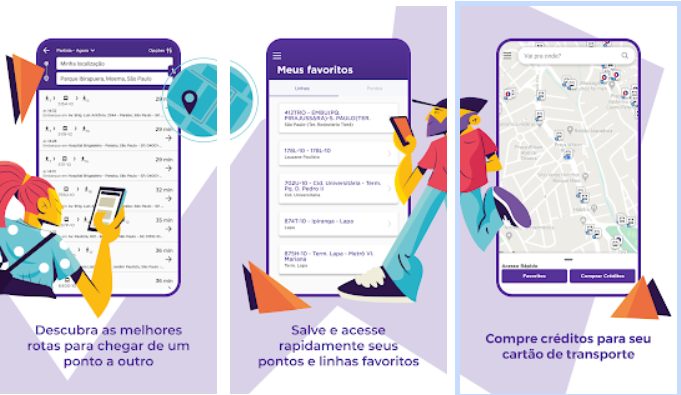
\includegraphics[width=0.4	\textwidth]{./04-figuras/cittamobi/cittamobi.png}
	\label{fig:cittamobi}
	\fonte{Loja de aplicativos do Android: PlayStore}
\end{figure}



%\subsection{Moovit}

\section{Transporte Individual Privado de Passageiros por Aplicativo}

A mobilidade vem mudando durante os anos, surgem novas maneiras e ferramentas para o uso da mobilidade, aplicativos como Uber, Cabify, BlaBlaCar, Yet Go, entraram no mercado e se tornaram ferramentas muito úteis, de grande uso, e ajudando tanto na mobilidade da população quanto no trânsito de muitas cidades, levando em consideração que pessoas que utilizam bastante deixam de ter a necessidade de possuir um carro para utilizar apenas esses serviços, baseado no conceito de consumo compartilhado que vimos anteriormente.

Esse novo conceito, essa nova abordagem de mobilidade é inserida nas cidades não apenas com as ferramentas citadas acima, mas outras iniciativas, como de universidades também tentam melhorar a mobilidade de seus determinados públicos através de aplicativos de carona solidária, pontos de parada de compartilhamento de corridas.

Inspiradas pelo crescente sucesso da Uber, surgiram startups visando de atuar de forma similar, mas voltados para o mercado de motoristas de táxi, algumas delas cresceram e se destacam por sua abrangência cada vez maior, como é o caso da Easy Taxi, empresa brasileira fundada em 2012 no Rio de Janeiro, presente em mais de 30 países e 420 cidades atualmente \cite{caronae}.
%texto não modificado

\subsection{Uber}
A história da Uber teve início quando seus fundadores, Garrett Camp e Travis Kalanick, em Paris, encontraram certa dificuldade para encontrar um táxi. Percebendo a demanda por transporte, os executivos resolveram criar uma plataforma que permitisse solicitar carros premium. A Uber foi fundada em 2009, na Califórnia, como um aplicativo para facilitar o acesso ao transporte.

A Uber chegou ao Brasil em 2014, com atuação no Rio de Janeiro. A segunda cidade a receber o aplicativo foi São Paulo, seguida por Belo Horizonte. Atualmente, mais de 100 cidades brasileiras contam com os serviços da empresa, realizados por 500 mil motoristas parceiros. 

%https://canaltech.com.br/empresa/uber/#:~:text=A%20hist%C3%B3ria%20da%20Uber%20teve,dificuldade%20para%20encontrar%20um%20t%C3%A1xi.&text=A%20Uber%20foi%20fundada%20em,facilitar%20o%20acesso%20ao%20transporte.

\begin{comment}
\subsection{99}
Fundada em 2012, a 99 é fruto da vontade de fazer diferente de três conhecidos geeks da internet brasileira: Ariel Lambrecht, Renato Freitas e Paulo Veras. Seis anos depois, fomos adquiridos pela DiDi, a maior plataforma de transporte por celular do mundo que atinge mais de 60\% da população mundial e cobre mais de mil cidades com um serviço de mobilidade cada dia melhor. Além do nosso trabalho constante pelo melhor serviço, perseguimos a missão de impactar positivamente a população, tornando o transporte mais barato, rápido e seguro para passageiros e o dia a dia mais rentável e tranquilo para motoristas através da tecnologia. E para que isso aconteça, damos poder de escolha para todos com as nossas categorias de serviço, que vão desde o 99Pop, com motoristas particulares em diversas cidades; até o 99Táxi, presente em todo o Brasil no modo tarifa cheia e desconto, que oferece a comodidade do táxi com valores até 30\% mais baixos; e o 99Top, um serviço premium com táxis de luxo. Assim, no brasil, conectamos 14 milhões de passageiros a 300 mil taxistas e motoristas e mudamos a vida de milhões de pessoas todos os dias, reinventando o seu jeito de ir e vir. 
%https://www.revelo.com.br/empresas/99taxis
    
\end{comment}

\subsection{Cabify}

Cabify é um dos grandes nomes no seguimento de aplicativos de viagem e deslocamento. A empresa é conhecida como uma multinacional de rede transporte, concorrente de outros serviços como, por exemplo, Uber e 99.

Em Cabify, a dinâmica é bem parecida com outros aplicativos de carona no mercado, seus usuários podem pedir por corridas para lugares determinados através de sua geolocalização.

No entanto, a plataforma conta com alguns diferenciais oferecendo o serviço de táxis e motoristas profissionais, além disso, é possível programar corridas de acordo com o dia e horário desejados, recurso que ainda foi pouco explorado por outros aplicativos. 

%https://canaltech.com.br/apps/cabify-o-que-e-como-funciona/%

\section{Viagens Compartilhadas por Aplicativos}
\subsection{BlaBlaCar}

 O BlaBlaCar é um aplicativo de caronas bastante utilizado para corridas intermunicipais, o valor fica a critério do caroneiro em negociação com o motorista. O aplicativo surgiu em meados de 2003 devido a necessidade de Fred (Fundador da BlaBlaCar) de ir visitar sua família no interior da França sem carro e com as passagens de trem esgotadas, ele pediu que sua irmã fosse buscá-lo, durante o caminho, ele notou que muitos carros andavam com muitos lugares desocupados, então, ele viu nessa situação um começo de um novo modal (BlaBlaCar, 2020).
        
O aplicativo é diferente dos citados acima por ser aberto para todos, basta realizar o cadastro e já pode compartilhar suas caronas. Comparado a outros aplicativos voltados à remuneração como Uber e 99, o BlaBlaCar costuma ter viagens mais longas, intermunicipais por exemplo, à um preço bem mais acessível. %texto escrito por mim

\subsection{Bynd}

A empresa foi criada no final de 2014 em decorrência de uma experiência pessoal de seus dois sócios-fundadores, Gustavo Bertazzola Graciteli e Leonardo Fernandes Libório, que fizeram uma viagem pelas Américas por 13 meses em um carro compartilhado com outras três pessoas. Após esse período sabático, ambos decidiram abandonar suas carreiras no mercado financeiro e iniciar um novo negócio. A ideia de criar a Bynd surgiu em uma palestra para empreendedores. na qual um dos diretores da Tecnisa (empresa do mercado imobiliário brasileiro) apresentou problemas que careciam de soluções mais eficazes; entre elas, a dificuldade em disponibilizar vagas de estacionamento aos funcionários da empresa. Assim, a Bynd surgiu para melhorar a taxa de ocupação dos veículos, melhorando a eficiência dos deslocamentos realizados por meio de carons corporativas.

% texto da Tesé André

O suporte da tecnologia da informação e comunicação foi imprescindivel para a que a Bynd oferecesse seus serviços, entre eles: a disponibilização do aplicativo para dispositivos móveis e do \textit{website}; a implementação de salas de bate-papo para facilitar a comunicação direta entre os usuários; a realização de atendimentos virtuais; o desenvolvimento dos mecanismos de premiação e de incentivos; as consultas às caronas disponíveis em tempo real; o envio de notificações, entre outros. Embora cientes da possibilidade de extrair dados de dispositivos da Internet das Coisas e de \textit{big data}, esses recursos ainda não foram implementados; contudo, os fundadores ressaltam que a previsibilidade e a confiabilidade são requisitos essenciais para a operação de seu modelo de negócio, e ambos são suportados pelas TIC. 

%texto da tese André

\subsection{Vemcar}

Desenvolvido na Universidade Federal do Rio Grande do Norte, o aplicativo Vemcar começou a ser desenvolvido em uma disciplina oferecida no curso de Engenharia de Software, logo após, o protótipo passou para a equipe da Superintendência de Informática da Universidade Federal do Rio Grande do Norte (SINFO), lá foi realizado toda a validação da ideia, surgimento dos requisitos e foram aplicadas as regras do um processo de software. No Vemcar somentes pessoas ligadas à universidade( professores, alunos, técnicos) podem utilizar o aplicativo.

%texto escrito por mim

\begin{figure}[!hbtp]
	\centering
	\caption{Aplicativo de Carona Solidária Vemcar}
	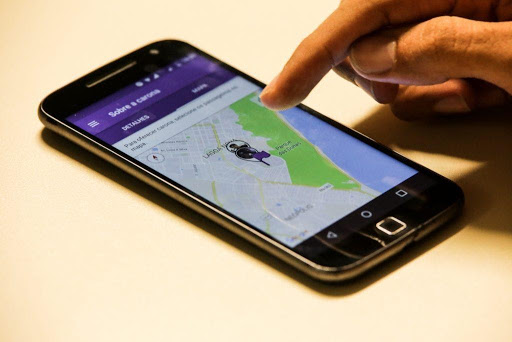
\includegraphics[width=0.5\textwidth]{./04-figuras/vemcar.jpg}
	\label{fig:tecnologia}
	\fonte{https://www.ufrn.br/imprensa/materias-especiais/2872/aplicativo-de-caronas-solidarias-da-ufrn-registra-mil-downloads-em-uma-semana}
\end{figure}


\subsection{Caronaê}

%mencionar trabalho da luísa e do artigo publicado sobre o aplcativo.

O Caronaê é um aplicativo de carona voltada para o ambiente universitário desenvolvido por alunos da Universidade Federal do Rio de Janeiro (UFRJ). O aplicativo está disponível para duas plataformas, Android e iOS. Em seu site oficial (CARONAÊ, 2020) diz que \textit{“O Caronaê é um sistema de código aberto, seguro e prático de caronas compartilhadas, criado com o objetivo de ser replicado em diferentes instituições e feito exclusivamente para a comunidade acadêmica das instituições integrantes da Rede Caronaê”}.

Dos pontos interessantes que o aplicativo oferece são, o uso exclusivo da comunidade acadêmica, a centralização das ofertas de carona, o aumento da taxa de ocupação dos veículos e pontos de carona para facilitar o encontro de caroneiro e carona. A Figura~\ref{fig:caronae} mostra a tela inicial do site do aplicativo de carona \textbf{Caronaê}.

\begin{figure}[!hbtp]
	\centering
	\caption{Aplicativo de Carona Solidária Caronaê}
	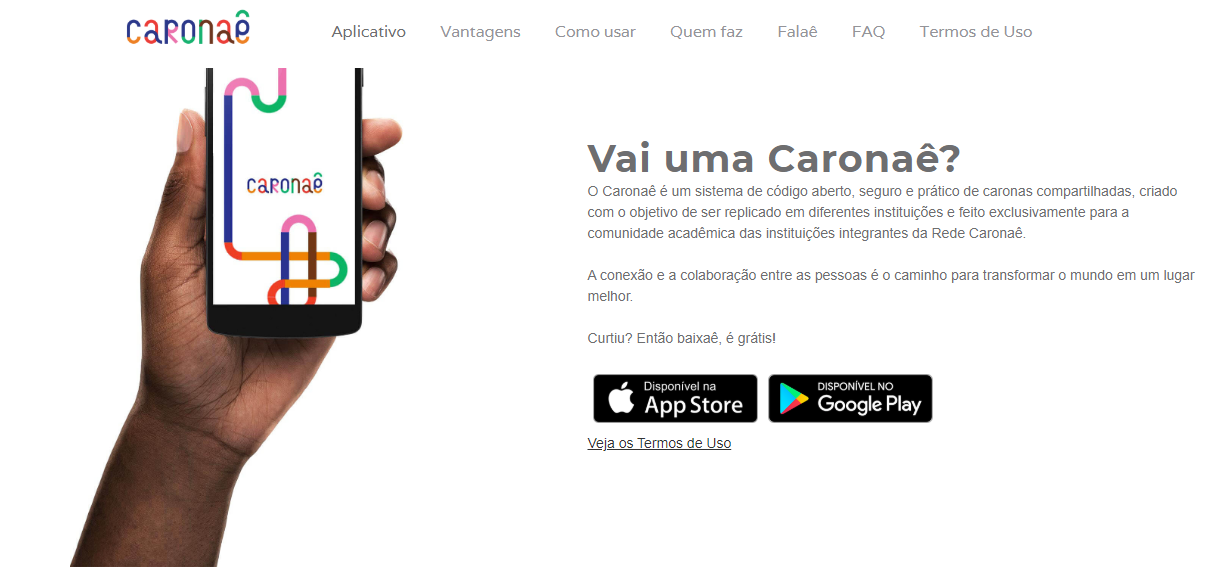
\includegraphics[width=0.8\textwidth]{./04-figuras/caronae.png}
	\label{fig:caronae}
	\fonte{https://caronae.org/index.html}
\end{figure}


%texto escrito por mim

\subsection{Waze Carpool}
Aplicativo das Empresas Waze, o \textit{Waze Carpool} é uma variante dos serviços da Waze que oferece compartilhamento de caronas entre seus usuários. O serviço oferecido pela empresa funciona através de um programa de parcerias. O aplicativo é bem dinâmico e intuitivo. A empresa aproveita os dados do aplicativo Waze para alimentar a dinâmica de navegação do Waze Carpool, como mostra a tela de grupos do aplicativo na Figura~\ref{fig:tela_grupos_wazecarpool}.

\begin{figure}[!hbtp]
	\centering
	\caption{Tela de grupos do aplicativo Waze Carpool}
	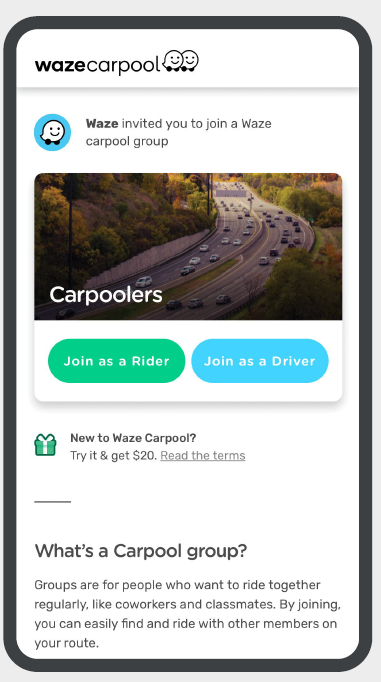
\includegraphics[width=0.25\textwidth]{./04-figuras/waze/Tela_de_grupos.png}
	\label{fig:tela_grupos_wazecarpool}
	\fonte{Programa de Parceria Brasil - Waze Carpool}
\end{figure}

A Waze oferece o serviço do aplicativo para diversas empresas que desejam incorporar a cultura das caronas entre seus empregados porque a empresa acredita que as caronas costumam aproximar mais as pessoas e criar momentos que no local de trabalho não existiriam.

O aplicativo tem uma dinâmica interessante, funciona a partir da criação de grupos, e os usuários destes grupos oferecem caronas entre si. Alunos de universidades como a UFRJ que por um tempo teve o seu próprio aplicativo de carona, o Caronaê, utilizam a ferramenta para pegar e oferecer a carona aos integrantes dos grupos que são criados e gerenciados por uma pessoa que ficar responsável pela comunicação da instituição com a empresa, o chamado "Embaixador".
% texto do material da waze 




\section{Veículos Compartilhados}
Na categoria de veículos compartilhados, separamos dois exemplos dos mais conhecidos com diferentes características cada. Há soluções desde compartilhamentos de bicicletas e automóveis.  %texto escrito por mim

Chips e cartões inteligentes ("\textit{smart-card}") são tecnologias bastante utilizadas nesse tipo de modelo de solução de mobilidade. Os chips utilizados em muitos casos para monitorar as bicicletas compartilhadas, e em algumas cidades, como Rennes na França, em 1998, utilizava os cartões inteligentes para a liberação das bicicletas nas estações.%mestrado da luisa

Aliás, Paris foi uma das primeiras cidades a utilizar os chamados sistemas de terceira geração, no qual a tecnologia utilizada é capaz de controlar o uso dos veículos em tempo real, GPS, cartões inteligentes, chips, todos, entram na lista dos dispositivos que possibilitam esse controle.

\subsection{Yellow}

Utilizando chips em seus veículos e QR Code para desbloquear seus veículos, a Yellow é uma startup brasileira de micromibilidade -- termo dado para veículos que servem para percorrer distâncias curtas -- que aluga bicicletas e partinetes elétricos fundada em 2017. Funcionando através de um serviço \textit{dockless}, ou seja, ao invés das bicicletas terem um ponto de estacionamento especifico, elas podem ser encontradas e deixadas em qualquer lugar que esteja dentro das áreas de atuação exibidas pelo aplicativo, podendo ser monitorada e controlada. 

Após o fim do uso, basta o usuário travar o cadeado que fica na bicicleta, que está pronta para o próximo usuário. A Yellow também utiliza o GPS, tanto para mostrar o trajeto percorrido pelo usuário quanto para apresentar onde estão as bicicletas no mapa. Na figura \ref{fig:yellow-app} é mostrado as áreas de atuação e a localização das bicicletas na cidade de São Paulo.

\begin{comment}
https://tecnoblog.net/286176/como-funciona-o-aluguel-de-bicicletas-e-patinetes-da-yellow/
\end{comment}

\begin{figure}[!hbtp]
	\centering
	\caption{Mapa do aplicativo Yellow na cidade de São Paulo}
	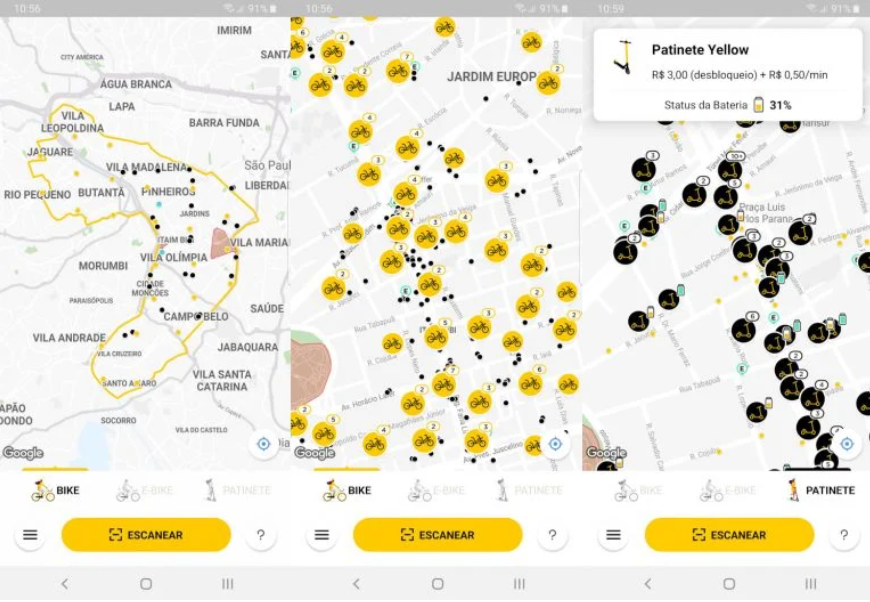
\includegraphics[width=0.6\textwidth]{./04-figuras/yellow/yellow.png}
	\label{fig:yellow-app}
	\fonte{https://tecnoblog.net/286176/como-funciona-o-aluguel-de-bicicletas-e-patinetes-da-yellow/} 
\end{figure}

\subsection{ZipCar}

Utilizando conceitos de \textit{Carsharing}, a empresa norte-americana que ainda não chegou com seus serviços no Brasil utiliza dos seus recursos tecnológicos -- aplicativo para dispositovos móveis -- para compartilhar carros entre seus usuários no estilo B2C (Business-to-Consumer). Semelhante a empresa Yellow, os usuários geralmente conseguem encontrar veículos próximos através de seus dispositivos móveis.

Segundo \cite{ballus-armet} os usuários do Zipcar precisam ao final do uso do veículo, devolvê-lo ao ponto de origem, algo que e chama de \textit{round-trip} ou ida e volta, modelo usado pela Zipcar. Outra empresa semelhante ao Zipcar é a Car2Go, divergindo no modelo de utilizaçao, na Car2Go o usuário deixa o veículo em uma localidade diferente por ser corridas chamadas \textit{one way}, ou seja, trecho único.

Ambos modelos de negócio estão relacionados a economia colaborativa e utilizam a plataforma da Internet, redes sociais, sistemas de informação e recursos tecnológico para oferecer o serviço e conectar seus usuários \cite{ballus-armet}. O aluguel são para pessoas que geralmente precisam de carros por poucas horas, % https://medium.com/@edselferri/o-case-zipcar-a7cbded4ba02#:~:text=Eles%20t%C3%AAm%20uma%20tecnologia%20sem,a%20torna%20um%20neg%C3%B3cio%20%C3%BAnico.
os clientes podem reservar um carro on-line e usar um cartão RFID chamado zipcard para entrar no carro reservado, passando o cartão no leitor perto do pára-brisa do motorista \cite{pearlson2009strategic} %\mnote{é um livro, precisa encontrar a página}.

%https://medium.com/@edselferri/o-case-zipcar-a7cbded4ba02#:~:text=Eles%20t%C3%AAm%20uma%20tecnologia%20sem,a%20torna%20um%20neg%C3%B3cio%20%C3%BAnico.
% texto copiado do site
Além de ter um serviço exclusivo, a Zipcar emprega tecnologia poderosa para dar suporte ao seu modelo de negócios \cite{pearlson2009strategic}. Eles têm uma tecnologia sem fio patenteada que é usada para monitorar a segurança do carro, o nível de feules, o uso por hora e outros recursos \cite{pearlson2009strategic}. A Zipcar desenvolveu um modelo de negócio único e apoiou-a com tecnologia apropriada, o que a torna um negócio único. Na figura \ref{fig:zipcar} mostra um usuário desbloqueando as portas do veículo da Zipcar.

\begin{figure}[!hbtp]
	\centering
	\caption{Como desbloquear seu Zipcar}
	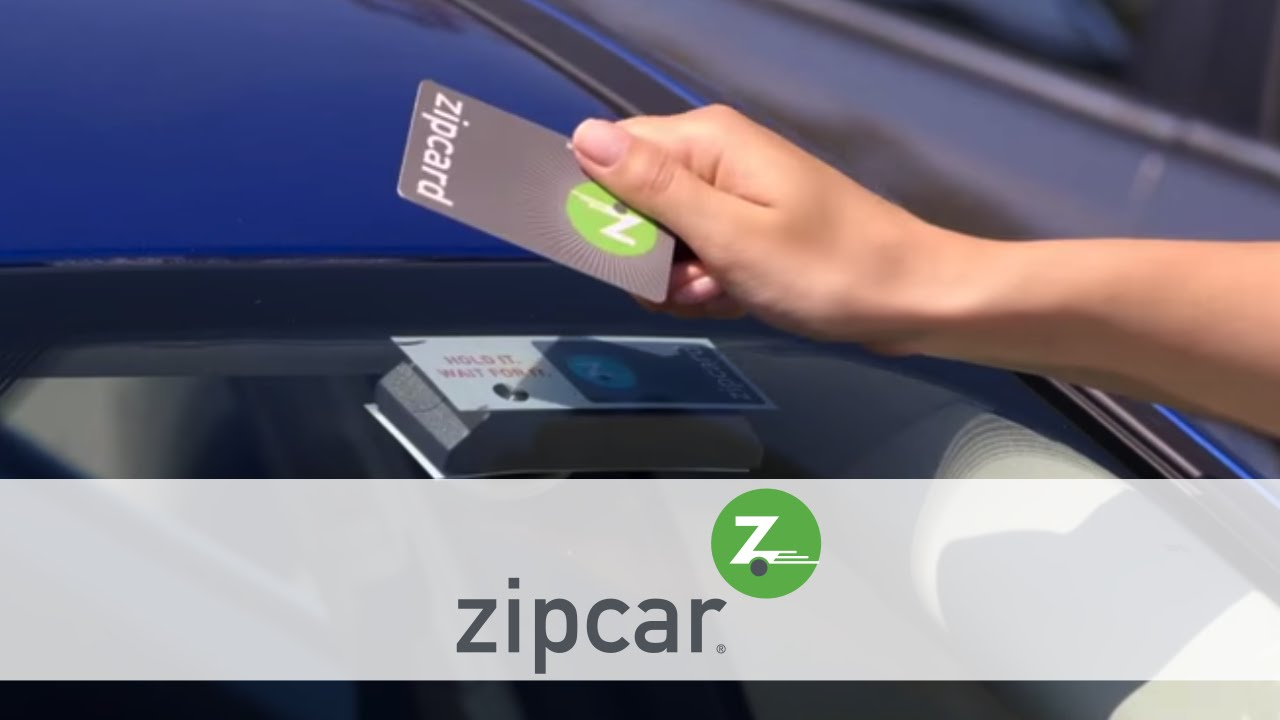
\includegraphics[width=0.8\textwidth]{./04-figuras/zipcar/zipcar.jpg}
	\label{fig:zipcar}
	\fonte{https://money.usnews.com/money/business-economy/articles/2008/06/05/5-keys-to-zipcars-success} %acesso: 13/04/2021 
\end{figure}


\begin{comment}
\section{Quadro Comparativo entre as soluções}
Depois de mostrar algumas das soluções existentes de mobilidade inteligente ao redor do mundo, vamos realizar uma comparação de qual solução será mais viável de ser implementada na Unifap levando em consideração o contexto local, as dificuldades de implementação e o questionário respondido pelo corpo docente e discente do Campus Macapá.

Levando em consideração o questionário que foi aplicado,logo de inicio, descartamos soluções de mobilidade inteligente que tem fins lucrativos e comerciais, como "Transporte Individual Privativo de Passageiros", além de não oferecerem nenhum serviço para o objetivo aqui proposto. Também, as "Orientações de Mobilidade" foram mencionadas para explanar sobre o tipo de mobilidade inteligente, porém, foge da ideia do projeto, pois não conseguiríamos oferecer o mínimo de garantia de segurança, praticidade e conforto.

As demais categorias mencionadas, "Viagens Compartilhadas" e "Veículos Compartilhados" foram analisados, e concluímos que seriam as mais viáveis. Excluímos as soluções privadas, que não garantiriam alguns requisitos mencionados no formulário, e analisamos 3 opções para oferecer, bicicletas compartilhadas, da categoria de veículos compartilhados e 2 soluções da categoria compartilhamento de corridas, Waze Carpool e Caronaê.

Os critérios foram baseados em cima das complexidade e contratempos que poderiam ter durante o processo de implementação, consideramos a infraestrutura institucional (UNIFAP) e da cidade de Macapá. Levamos em consideração também o custo tanto pro usuário, quanto pra universidade em organizar, gerenciar e manter os serviços da solução, além de necessidade futura de estar preparada para oferecer o serviço com qualidade independente do volume de dados. Soluções que já dispõem sua própria infraestrutura tecnológica parece atraente, porém, a maioria não fica dentro dos requisitos da comunidade da Unifap.

No quadro \ref{tab:quadro-solusdemobilidade} resume as características e modelos de negócios citados, apresentando algumas funcionalidades e regra de negócio de cada solução, além de expor quais soluções estão disponíveis para uso conforme as necessidades locais. O aplicativo Caronaê aparece como opção por ser de código aberto, e disponibiliza pelo GitHub a plataforma mobile, sua área administrativa e demais serviços, já o Waze Carpool nos da a possibilidade de criar grupos fechados, nos da todo o aparato tecnologico e as aplicações, nos dando apenas a responsabilidade de gerenciar os usuários e grupos. 
% Please add the following required packages to your document preamble:
% \usepackage{graphicx}
% \usepackage[table,xcdraw]{xcolor}
% If you use beamer only pass "xcolor=table" option, i.e. \documentclass[xcolor=table]{beamer}
% \usepackage{lscape}
\begin{landscape}
\begin{quadro}[]
\caption{Soluções de mobilidade}
\label{tab:quadro-solusdemobilidade}
\resizebox{1.5\textwidth}{!}{%
\begin{tabular}{|l|l|l|l|l|l|l|l|l|l|l|l|}
\hline
\multicolumn{12}{|c|}{Soluções de mobilidade} \\ \hline
\multicolumn{1}{|c|}{Nome} &
  Categoria &
  \multicolumn{1}{c|}{\begin{tabular}[c]{@{}c@{}}Oferecer/Solicitar\\ Caronas\end{tabular}} &
  \multicolumn{1}{c|}{Proprietário} &
  \multicolumn{1}{c|}{\begin{tabular}[c]{@{}c@{}}Ambiente\\ administrativo \\ disponível a terceiros\end{tabular}} &
  \multicolumn{1}{c|}{Autenticação} &
  \multicolumn{1}{c|}{GPS} &
  \multicolumn{1}{c|}{\begin{tabular}[c]{@{}c@{}}Utiliza remuneração\\ no aplicativo\end{tabular}} &
  Plataforma &
  \begin{tabular}[c]{@{}l@{}}Identificação do \\ usuário\end{tabular} &
  Código aberto &
  Infraestrutura \\ \hline
Waze &
  \begin{tabular}[c]{@{}l@{}}Orientação \\ de mobilidade\end{tabular} &
  Não &
  Waze Mobile &
  Não &
  \begin{tabular}[c]{@{}l@{}}Qualquer pessoa \\ que realizar o cadastro\end{tabular} &
  {\color[HTML]{000000} Sim} &
  Não &
  Android IOS &
  Conta cadastrada &
  Não &
  Própria \\ \hline
Cittamobi &
  \begin{tabular}[c]{@{}l@{}}Orientação \\ de mobilidade\end{tabular} &
  Não &
  Cittati &
  Não &
  \begin{tabular}[c]{@{}l@{}}Qualquer pessoa \\ que realizar o cadastro\end{tabular} &
  Sim &
  Não &
  Android IOS &
  Conta cadastrada &
  Não &
  Própria \\ \hline
Moovit &
  \begin{tabular}[c]{@{}l@{}}Orientação \\ de mobilidade\end{tabular} &
  Não &
  Moovit Inc. &
  Não &
  \begin{tabular}[c]{@{}l@{}}Qualquer pessoa \\ que realizar o cadastro\end{tabular} &
  Sim &
  Não &
  Android IOS &
  Conta cadastrada &
  Não &
  Própria \\ \hline
Google Maps &
  \begin{tabular}[c]{@{}l@{}}Orientação \\ de mobilidade\end{tabular} &
  Não &
  Google &
  Não &
  \begin{tabular}[c]{@{}l@{}}Qualquer pessoa \\ que realizar o cadastro\end{tabular} &
  Sim &
  Não &
  Android IOS &
  Conta cadastrada &
  Não &
  Própria \\ \hline
Uber &
  \begin{tabular}[c]{@{}l@{}}Transporte índividual\\ privado de passageiros\end{tabular} &
  Não &
  Uber Technologies Inc. &
  Não &
  \begin{tabular}[c]{@{}l@{}}Qualquer pessoa \\ que realizar o cadastro\end{tabular} &
  Sim &
  Sim &
  Android IOS &
  Conta cadastrada &
  Não &
  Própria \\ \hline
99 &
  \begin{tabular}[c]{@{}l@{}}Transporte índividual\\ privado de passageiros\end{tabular} &
  Não &
  Didi Chuxing &
  Não &
  \begin{tabular}[c]{@{}l@{}}Qualquer pessoa \\ que realizar o cadastro\end{tabular} &
  Sim &
  Sim &
  Android IOS &
  Conta cadastrada &
  Não &
  Própria \\ \hline
Blablacar &
  Viagens compartilhadas &
  Sim &
  Comuto SA &
  Não &
  \begin{tabular}[c]{@{}l@{}}Qualquer pessoa \\ que realizar o cadastro\end{tabular} &
  Não &
  Sim &
  Android IOS &
  Conta cadastrada &
  Não &
  Própria \\ \hline
Yellow &
  Veículos compartilhados &
  Não &
  Grow &
  Não &
  \begin{tabular}[c]{@{}l@{}}Qualquer pessoa \\ que realizar o cadastro\end{tabular} &
  Sim &
  Sim &
  Android IOS &
  Conta cadastrada &
  Não &
  Própria \\ \hline
Cabify &
  Viagens compartilhadas &
  Não &
  Juan de Antonio &
  Não &
  \begin{tabular}[c]{@{}l@{}}Qualquer pessoa \\ que realizar o cadastro\end{tabular} &
  Sim &
  Sim &
  Android IOS &
  Conta cadastrada &
  Não &
  Própria \\ \hline
Bynd &
  Viagens compartilhadas &
  Não &
   &
  Não &
  \begin{tabular}[c]{@{}l@{}}Qualquer pessoa \\ que realizar o cadastro\end{tabular} &
  Sim &
  Sim &
  Android IOS &
  Conta cadastrada &
  Não &
  Própria \\ \hline
Vemcar &
  Viagens compartilhadas &
  Sim &
  UFMG &
  Não &
  \begin{tabular}[c]{@{}l@{}}Somente alunos da \\ UFMG\end{tabular} &
  Sim &
  Recompensas &
  Android &
  \begin{tabular}[c]{@{}l@{}}Sistema de Gestão\\ da UFMG\end{tabular} &
  Não &
  UFMG \\ \hline
ZipCar &
  Veículos compartilhados &
  Não &
  Avis Budget Group &
  Não &
  \begin{tabular}[c]{@{}l@{}}Qualquer pessoa \\ que realizar o cadastro\end{tabular} &
  Sim &
  Sim &
  Android IOS &
  Conta cadastrada &
  Não &
  Própria \\ \hline
Caronaê &
  Viagens compartilhadas &
  Sim &
  UFRJ &
  Sim &
  \begin{tabular}[c]{@{}l@{}}Somente alunos da \\ UFRJ\end{tabular} &
  Não &
  Não &
  Android IOS &
  \begin{tabular}[c]{@{}l@{}}Sistema de Gestão \\ da UFRJ\end{tabular} &
  %\cellcolor[HTML]{FFFC9E}
  Sim &
  UFRJ \\ \hline
Waze Carpool &
  Viagens compartilhadas &
  Sim &
  Waze Mobile &
  %\cellcolor[HTML]{FCFF2F}
  Sim &
  \begin{tabular}[c]{@{}l@{}}Qualquer pessoa \\ que realizar o cadastro\end{tabular} &
  Sim &
  Sim &
  Android IOS &
  Conta cadastrada &
  Não &
  Própria \\ \hline
\end{tabular}%
}
\end{quadro}
\end{landscape}


%%%%%%%%%5
\begin{comment}
	\mnote{Patrícia: vais ter que expandir esse capítulo. Se nao me engano a gnt tnha conversado sobre falar de algumas soluções de mobilidade inteligente existentes, vai ser importante para o teu argumento. Vou criar uma seção somente para "veículos compartilhados", ou seja, app de carona, uber, etc, depois vc organiza e vê se é o melhor termo e cria as demais seções.}
    %
    
    %
	\mnote{Patrícia: vamos pensar se colocamos essa seção na próxima seção de proposta e resultados preliminares.}
    %
\end{comment}
%%%%%%%%
\end{comment}

